% !TeX program = lualatex
\documentclass[../skript/main.tex]{subfiles}
\begin{document}
	
\chapter{Einführung}\label{chap:einfuehrung}
\section{Der Begriff Informatik}

Das Wort \textbf{Informatik} setzt sich aus zwei Teilen zusammen: \emph{Information} und \emph{Automatik}. 
Ursprünglich wurde der Begriff in den 1950er Jahren in Frankreich geprägt 
(\glqq informatique\grqq{}) und fand später auch im deutschsprachigen Raum Verbreitung. 
In anderen Sprachen wird der Bereich meist \glqq Computer Science\grqq{} genannt, 
was die technische Seite stärker betont. 

\subsection{Information}
Der erste Bestandteil, \emph{Information}, bezieht sich auf Daten, die eine Bedeutung tragen. 
Information ist also nicht einfach nur eine Ansammlung von Zeichen oder Zahlen, 
sondern sie entsteht erst durch die \emph{Interpretation} von Daten in einem bestimmten Kontext.  
Beispielsweise ist die Zahl \glqq 42\grqq{} zunächst nur ein einzelner Wert.
Wird sie jedoch im Zusammenhang mit einer Temperaturangabe, einem Alter oder einem Ergebnis verstanden, wird daraus eine Information.  
Die Informatik beschäftigt sich also damit, Informationen \emph{darzustellen}, 
\emph{zu speichern}, \emph{zu übertragen} und \emph{zu verarbeiten}.

\subsection{Automatik}
Der zweite Bestandteil, \emph{Matik} (von Automatik), bedeutet, dass diese Informationsverarbeitung 
durch Maschinen – insbesondere Computer – automatisiert geschieht.  
Ein zentrales Ziel der Informatik ist es, Verfahren zu entwickeln, die es ermöglichen, 
Informationen mithilfe von Computern effizient und zuverlässig zu verarbeiten. 
Dazu gehören das Erstellen von Programmen, das Entwerfen von Algorithmen 
sowie die Entwicklung von Systemen, die Informationen ohne manuelle Eingriffe verarbeiten können.

\section{Bedeutung der Informatik}
Die Informatik kann somit als \emph{Wissenschaft von der systematischen Verarbeitung von Informationen, insbesondere mit Hilfe von Computern}, verstanden werden. 
Sie ist nicht nur eine technische Disziplin, sondern verbindet Elemente aus 
Mathematik, Ingenieurwissenschaften, Logik und zunehmend auch Sozial- und Geisteswissenschaften. 
Heute prägt die Informatik nahezu alle Bereiche des täglichen Lebens: 
von Smartphones und dem Internet über moderne Autos bis hin zu Medizin, Wirtschaft und Wissenschaft.

\section{Was tun eigentlich Computer?}

Computer \emph{verarbeiten Daten}. Sie führen Berechnungen aus, speichern, übertragen und strukturieren Daten — aber sie „verstehen“ keine Bedeutung im menschlichen Sinn. Bedeutung (Information) entsteht erst beim Menschen (oder in einem Modell), wenn Daten in \emph{Kontext} gesetzt werden. Der Kernprozess ist daher zweistufig:

\begin{enumerate}
	\item \textbf{Repräsentation:} Aus \emph{Information} werden \emph{Daten}, indem wir festlegen, wie etwas als Zeichen/Zahlen (Bits) dargestellt wird.
	\item \textbf{Abstraktion:} Aus \emph{Daten} wird (wieder) \emph{Information}, indem wir Details weglassen, strukturieren und die Daten in einem Modell deuten.
\end{enumerate}

\subsection{Von Information zu Daten: Repräsentation}

\emph{Repräsentation} bedeutet: Wir legen eine \textbf{Abbildung} fest, die etwas Bedeutungsvolles (Information) in ein \textbf{Datenformat} überführt, das der Computer verarbeiten kann.
Formal kann man das als Funktion auffassen:
\[
\mathrm{rep}:\ \text{Information} \times \text{Kontext} \;\to\; \text{Daten (Bits)}.
\]


\subsection{Von Daten zu Information: Abstraktion}

\emph{Abstraktion} bedeutet: Wir \textbf{interpretieren} Daten in einem passenden Modell und \textbf{lassen Details weg}, die für die Fragestellung nicht nötig sind. So entsteht Bedeutung.
Formal:
\[
\mathrm{abs}:\ \text{Daten (Bits)} \times \text{Modell/Kontext} \;\to\; \text{Information}.
\]

\begin{figure}[H]
	\centering
	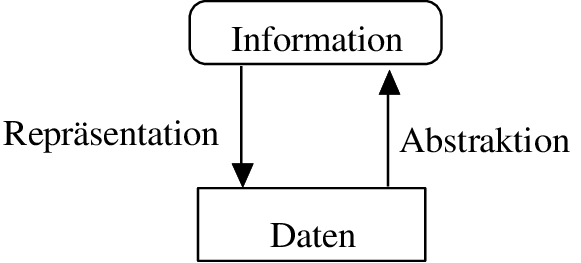
\includegraphics[width=0.55\textwidth]{info-daten.png}% ggf. Pfad anpassen
	\caption{Wechselspiel zwischen Repräsentation (Information → Daten) und Abstraktion (Daten → Information).}
	\label{fig:info-daten}
\end{figure}

\section{Bits und Bytes}

Ein \textbf{Bit} (binary digit) ist die kleinste Informationseinheit im Rechner: Es kann genau zwei Zustände annehmen, meist als \texttt{0} und \texttt{1} notiert. Physikalisch werden Bits z.\,B. durch zwei Spannungsniveaus, magnetische Ausrichtungen oder Lichtimpulse realisiert.

Einzelne Bits sind für die Verarbeitung jedoch zu fein. Deshalb werden Bits zu \textbf{Gruppen} zusammengefasst und \emph{gruppenweise} gelesen/geschrieben:

\begin{itemize}
	\item \textbf{Byte} = 8 Bit (heute die gebräuchlichste Grundeinheit; in den meisten Architekturen zugleich die \emph{kleinste adressierbare Einheit}).
	\item \textbf{Nibble} = 4 Bit (halbes Byte; nützlich z.\,B. bei Hexadezimaldarstellungen).
	\item \textbf{Wort (Word)} = \emph{architekturabhängige} Arbeitsbreite der CPU (typisch 16, 32 oder 64 Bit).
	\item \textbf{Doppelwort/Quadwort} = Vielfache der Wortbreite (z.\,B. 32/64/128 Bit).
\end{itemize}

\subsection{Wer bestimmt die Lesegruppen?}
\textbf{Hardware:} Die \emph{Register- und ALU-Breite} eines Prozessors legt fest, wie viele Bits er in einem Schritt besonders effizient verarbeiten kann (z.\,B. 32-Bit oder 64-Bit). Auch \emph{Datenbus} und \emph{Cache-Zeilengrößen} begünstigen das Holen/Speichern ganzer Bytes-, Wort- oder Mehrfach-Wort-Blöcke. Moderne CPUs können zusätzlich mit Vektor\-/SIMD-Einheiten noch größere Pakete (z.\,B. 128/256/512 Bit) auf einmal verarbeiten.

\textbf{Software/Betriebssystem:} Damit die Hardwarebreite genutzt werden kann, muss das \emph{Betriebssystem} die Architektur unterstützen (32-Bit- oder 64-Bit-Modus, Treiber, Systembibliotheken, ABI). Ein 64-Bit-Prozessor entfaltet seine Vorteile erst vollständig mit einem 64-Bit-Betriebssystem und passenden Programmen; andernfalls arbeitet er im 32-Bit-Kompatibilitätsmodus.

\paragraph{Beispiele.}
\begin{itemize}
	\item \textbf{32-Bit-System:} Die CPU arbeitet effizient mit 32-Bit-Wörtern (z.\,B. \texttt{int32}); Zeiger/Adressen sind 32 Bit breit. Daten werden häufig in 32-Bit-Schritten geladen/geschrieben, obwohl der Speicher byteweise adressiert wird.
	\item \textbf{64-Bit-System:} Register und Zeiger sind 64 Bit breit. Das System kann größere Zahlenbereiche adressieren und pro Schritt breitere Daten verarbeiten; trotzdem bleiben Bytes (8 Bit) die kleinste adressierbare Einheit.
\end{itemize}
\newpage
\section{Größe der Daten}

\begin{center}
	\begin{tabular}{r c l c l l}
		$1~\text{k}$ & = & $1024~\text{Bit}$ & = & $2^{10}$  & (k = Kilo)\\
		$1~\text{M}$ & = & $1024 \times 1024~\text{Bit}$ & = & $2^{20}$  & (M = Mega)\\
		$1~\text{G}$ & = & $1024 \times 1024 \times 1024~\text{Bit}$ & = & $2^{30}$  & (G = Giga)\\
		$1~\text{T}$ & = & $1024 \times 1024 \times 1024 \times 1024~\text{Bit}$ & = & $2^{40}$  & (T = Tera)\\
		$1~\text{P}$ & = & $1024 \times 1024 \times 1024 \times 1024 \times 1024~\text{Bit}$ & = & $2^{50}$  & (P = Peta)\\
		$1~\text{E}$ & = & $1024 \times 1024 \times 1024 \times 1024 \times 1024 \times 1024~\text{Bit}$ & = & $2^{60}$  & (E = Exa)\\
		$1~\text{Z}$ & = & $1024 \times 1024 \times 1024 \times 1024 \times 1024 \times 1024 \times 1024~\text{Bit}$ & = & $2^{70}$  & (Z = Zetta)\\
		$1~\text{Y}$ & = & $1024 \times 1024 \times 1024 \times 1024 \times 1024 \times 1024 \times 1024 \times 1024~\text{Bit}$ & = & $2^{80}$  & (Y = Yotta)\\
	\end{tabular}
\end{center}

\section{Textdarstellung}

\paragraph{Von ASCII zu Unicode — warum überhaupt?}
Frühe Computersysteme nutzten \textbf{ASCII} (American Standard Code for Information Interchange, 1960er Jahre). ASCII ist ein 7-Bit-Zeichensatz mit 128 Zeichen: lateinische Grundbuchstaben A–Z/a–z, Ziffern, Satzzeichen und Steuerzeichen (z.\,B. Zeilenumbruch). Für englischen Text genügte das, \emph{aber}:
Umlaute (ä, ö, ü), Akzente (é), das Euro-Zeichen (€), kyrillisch (Ж), griechisch (Ω), arabisch ({\arabicfont م}), asiatische Schriften ({\cjkfont 日}), Emojis ({\emojifont 😊}) \emph{fehlten}.
„é“ (NFC) vs. „e\combacute“ (NFD) bzw. „e + \dottedcircle\combacute“.
\emph{fehlten}.


Als Übergang entstanden viele \textbf{„erweiterte ASCII“-Codepages} (8-Bit, 256 Zeichen), z.\,B. \texttt{ISO-8859-1}, \texttt{Windows-1252}, \texttt{KOI8-R}. Jede deckte \emph{einen} Sprachraum ab. Ergebnis: Inkompatibilitäten (sogenanntes \emph{Mojibake}), weil dieselben Bytewerte je nach Codepage andere Zeichen bedeuten.

\textbf{Unicode} (seit 1991) löst dieses Grundproblem: \emph{ein} weltweiter Zeichensatz für \emph{alle} Schriftsysteme, Symbole, technische Zeichen und Emojis. Ziel: \emph{„Jedem Zeichen ein eindeutiger Codepunkt“} — unabhängig von Sprache, Plattform oder Anwendung.

\paragraph{Begriffe sauber trennen}
\begin{itemize}
	\item \textbf{Codepunkt} (Unicode): eine Nummer in der Form \texttt{U+XXXX} (z.\,B. \texttt{U+00E4} = „ä“, \texttt{U+20AC} = „€“, \texttt{U+1F60A} = „😊“).
	\item \textbf{Kodierung} (Encoding): konkrete Regel, wie Codepunkte in \emph{Bytes} umgesetzt werden (z.\,B. UTF-8, UTF-16, UTF-32).
	\item \textbf{Graphem-Cluster}: was der Mensch als „ein Zeichen“ wahrnimmt (z.\,B. „e“ + kombinierender Akzent \texttt{U+0301} $\to$ „é“, oder Familien-Emoji aus mehreren Codepunkten).
\end{itemize}

\paragraph{Wichtige Unicode-Kodierungen}
\begin{itemize}
	\item \textbf{UTF-8} (variabel, 1–4 Byte pro Codepunkt): ASCII-Zeichen bleiben 1 Byte (abwärtskompatibel), alle anderen werden als 2–4 Byte kodiert. Heutzutage Standard im Web, in Dateien und Schnittstellen.
	\item \textbf{UTF-16} (variabel, 2 oder 4 Byte): Basis-Mehrsprachige Ebene (BMP) meist 2 Byte; Supplementärzeichen (z.\,B. viele Emojis) als Surrogatpaare (4 Byte). Achtung auf Byte-Reihenfolge (\emph{Endianness}) und optionales \emph{BOM}.
	\item \textbf{UTF-32} (fix 4 Byte): einfacher, aber speicherintensiv; praktisch v.\,a. intern in manchen Systemen.
\end{itemize}

\paragraph{Historische Entwicklung in Kürze}
\begin{description}
	\item[1963] ASCII (7-Bit) standardisiert Grundzeichen und Steuerzeichen.
	\item[1980er] Viele 8-Bit-Codepages (\texttt{ISO-8859-x}, \texttt{Windows-125x}) — regionale Lösungen, wenig kompatibel.
	\item[1991+] Unicode-Projekt: \emph{ein} universeller Zeichensatz; Trennung von \emph{Zeichen} (Codepunkte) und \emph{Kodierung} (UTFs).
	\item[2000er+] UTF-8 setzt sich global durch (Internet, Linux/Unix, moderne Apps und Protokolle).
\end{description}

\paragraph{Wie wird Unicode praktisch genutzt?}
\begin{itemize}
	\item \textbf{Dateien und Protokolle:} Textdateien, JSON, HTML, E-Mails, Datenbanken — fast überall ist UTF-8 üblich. Wichtig: \emph{Encoding angeben} (z.\,B. HTTP \texttt{Content-Type}, HTML \texttt{<meta charset="utf-8">}, DB-Kollation).
	\item \textbf{Betriebssysteme:} Dateinamen und Konsolen sind (je nach System) Unicode-fähig; moderne Terminals verstehen UTF-8.
	\item \textbf{Programmiersprachen:} Python, Java, JavaScript, C\# u.\,a. arbeiten intern mit Unicode-Zeichenketten; I/O nutzt meist UTF-8.
\end{itemize}

%\chapter{Einführung}
%Dieses Skript dient als Einführung in zentrale Konzepte der Informatik.
%Wir verwenden das \texttt{subfiles}-Paket, um Kapitel \emph{modular} zu pflegen.
%\begin{itemize}
%  \item Kompiliere \texttt{main.tex} für das Gesamtwerk.
%  \item Oder kompiliere \texttt{chapters/einfuehrung.tex} direkt, wenn du nur dieses Kapitel testen möchtest.
%\end{itemize}
%
%\section{Organisation des Projekts}
%Die Verzeichnisstruktur ist wie folgt angelegt:
%\begin{verbatim}
%latex-book-subfiles/
%├── main.tex
%├── chapters/
%│   ├── einfuehrung.tex
%│   └── zweierkomplement.tex
%├── appendix/
%│   └── anhang.tex
%└── figures/
%\end{verbatim}
%
%\section{Bilder und Pfade}
%Für den Hauptlauf ist \verb|\graphicspath{{figures/}}| gesetzt.
%In Subfiles kann mit \verb|\graphicspath{{\subfix{../figures/}}}| gearbeitet werden,
%damit Einzelläufe ebenfalls funktionieren.

\end{document}
